%! TEX root = icml_drau.tex
\section{Experiments}
\label{sec:exp}
%! TEX root = icml_drau.tex
\begin{figure*}[ht]
	\centering
	\includegraphics[width=\textwidth]{figs_data/full_results.pdf}
	\label{fig:full_results}
	\caption{Results on a variety of environments}
\end{figure*}

The experiment set provided here is specifically aimed at showing that
the proposed method DAU can operate efficiently on a wide range of time
discretizations, without specific tuning, while standard deep Q-learning
approaches cannot. DAU is compared to DDPG in continuous action settings and to DQN in
discrete action settings. \TODO{(We only test off-policy
algorithms.)}

In all settings, we use the learning algorithm described in
Alg.~\ref{alg:dau} and \TODO{supplementary, algo 1}. The variants of DDPG and DQN
used are described in the supplementary material, as well as all the hyperparameters
used. To make comparison fair, we use the properly rescaled discount
factor $\gamma_\deltat$ and reward $r_\deltat$ from \eqref{eq:def-gamma},
as well as scaled learning rates, for DDPG and DQN. \TODO{NDY not
convincing: precisely because DDPG and DQN are not invariant, they might
benefit from a different scaling.}

Let us stress that the quantities plotted are rescaled to make comparison
possible across different timesteps. For example,
return results are given in term of discretized return $R_\deltat$ as defined in \eqref{eq:discretized-return},\footnote{This mostly amounts to scaling rewards
by a factor $\deltat$ when this scaling is not naturally done in the environment. Environment-specific
details are given in the supplementary material.} and, most notably, time elapsed is always given in
normalized epochs (physical time), i.e. the true number of epochs multiplied by the
discretization timestep.


\paragraph{Qualitative experiments: Visualizing policies and values}
To provide qualitative results, and check that robustness to time
discretization is provided both in term of raw return results, but also in term
of convergence of approximate value function and policies, we first provide results on the simple pendulum environment
from the OpenAI Gym classic control suite.  This environment's state space is of dimension $2$. A visualization of both the learnt value and policy functions is obtained by plotting for each point of the phase diagram $(\theta, \dot{\theta})$ its value and policy. results are presented in
Fig.~\ref{fig:pend} for the policy function and in Fig.\TODO{ref} in Supplementary \TODO{ref} for the value function.

We observe the learnt policy at several instants in physical time (or normalized epochs) during training, for various time discretizations $\deltat$, for both DAU and DDPG. With DAU, the agent's policy quickly converges for every time discretization without specific hyperparameter tuning. On the contrary, with DDPG, the agent is only able to learn for the two highest time discretization, and learning gets harder as $\deltat$ decreases.

\paragraph{Quantitative experiments}
We benchmark DAU against DDPG on classic control benchmarks: Pendulum, Cartpole, BipedalWalker, Ant and Half-Cheetah environments from OpenAI Gym. For Pendulum and Ant, DDPG is able to learn for the highest $\deltat$ but fails for the others, while DAU remains reasonably invariant to the time discretization. On Bipedal Walker, DDPG is never able to learn while DAU is achieving decent performance for all the $\deltat$'s. On Cartpole and Half Cheetah, results are less clear. On Cartpole, noise dominates, which makes interpretation difficult. On Half Cheetah, DAU is not clearly more invariant to time discretization than DDPG. This could be explained by the multiple suboptimal regimes that coexist in the half cheetah environment (walking on the head, walking on the back), and that DAU may fail to correctly weight the performance of each regime (as explained in Section \ref{sec:discussions}).

% \begin{figure}[h]
%   \centering
%   \includegraphics[width=\columnwidth]{figs_data/cartpole_lc.png}
%   \caption{Cartpole}
%   \label{fig:cartpole-lc}
% \end{figure}

% \begin{figure}[h]
%   \centering
%   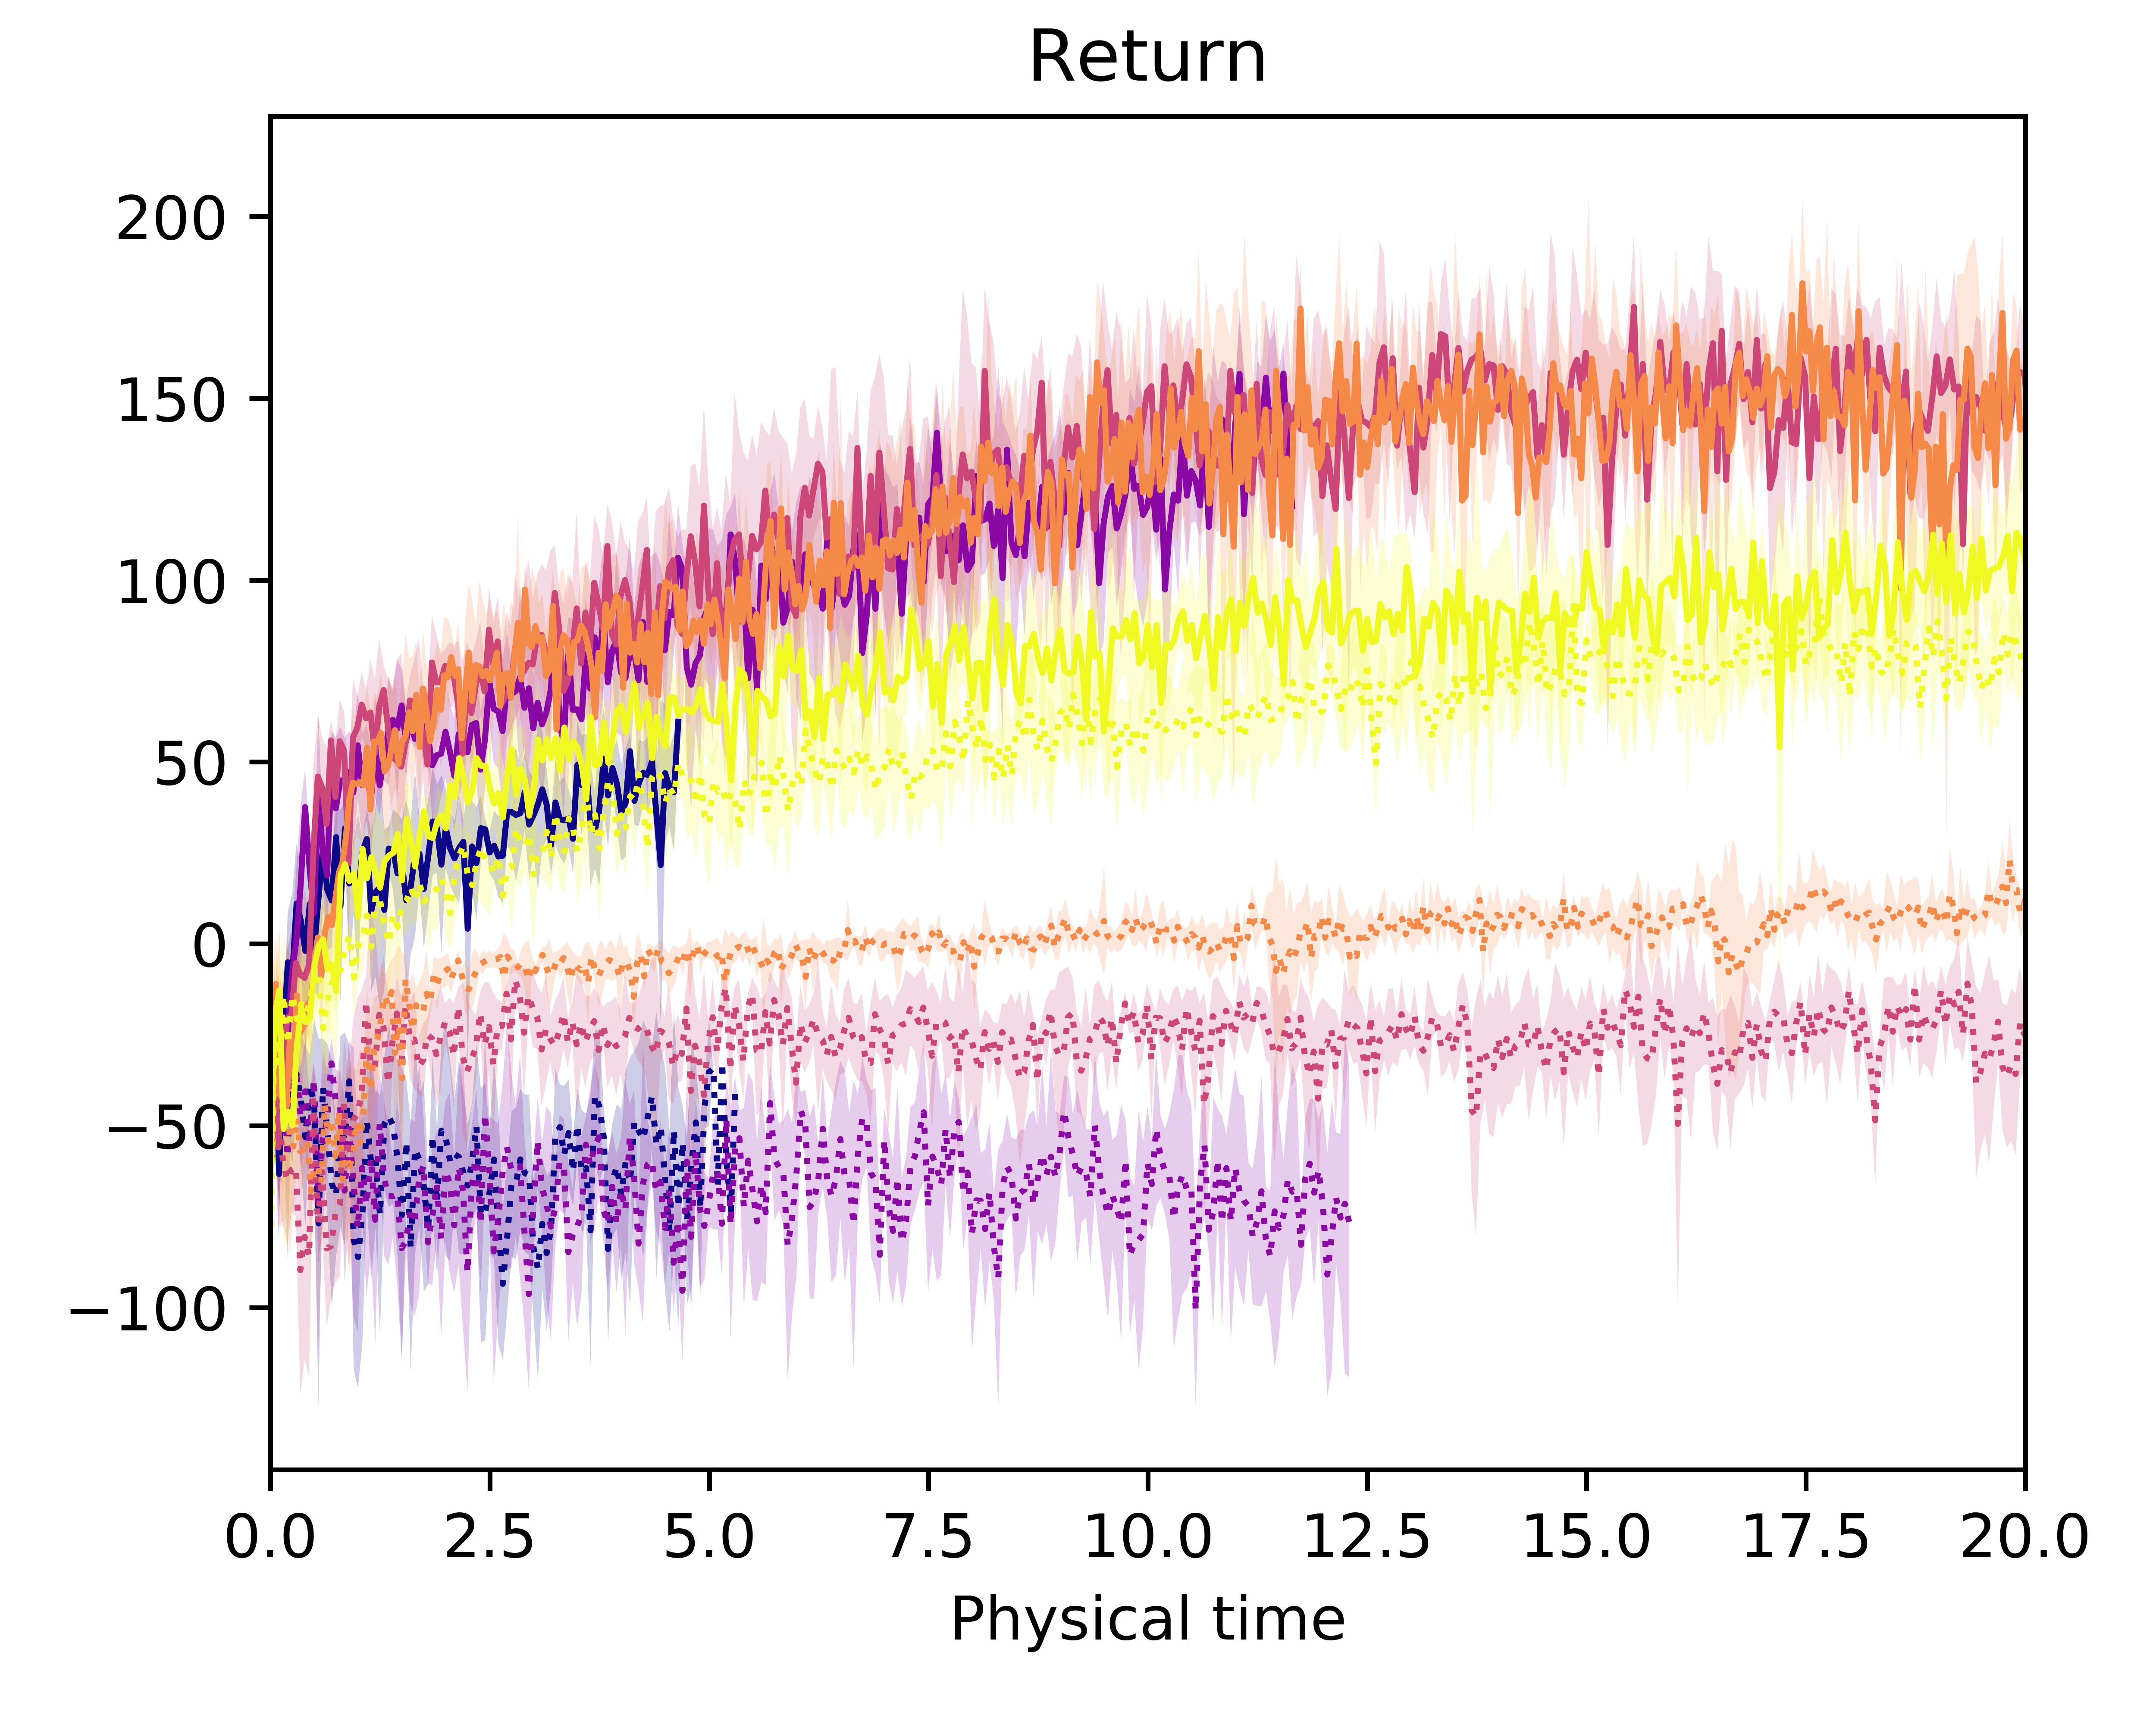
\includegraphics[width=\columnwidth]{figs_data/ant_lc.png}
%   \caption{Ant}
%   \label{fig:ant-lc}
% \end{figure}
% 
% \begin{figure}[h]
%   \centering
%   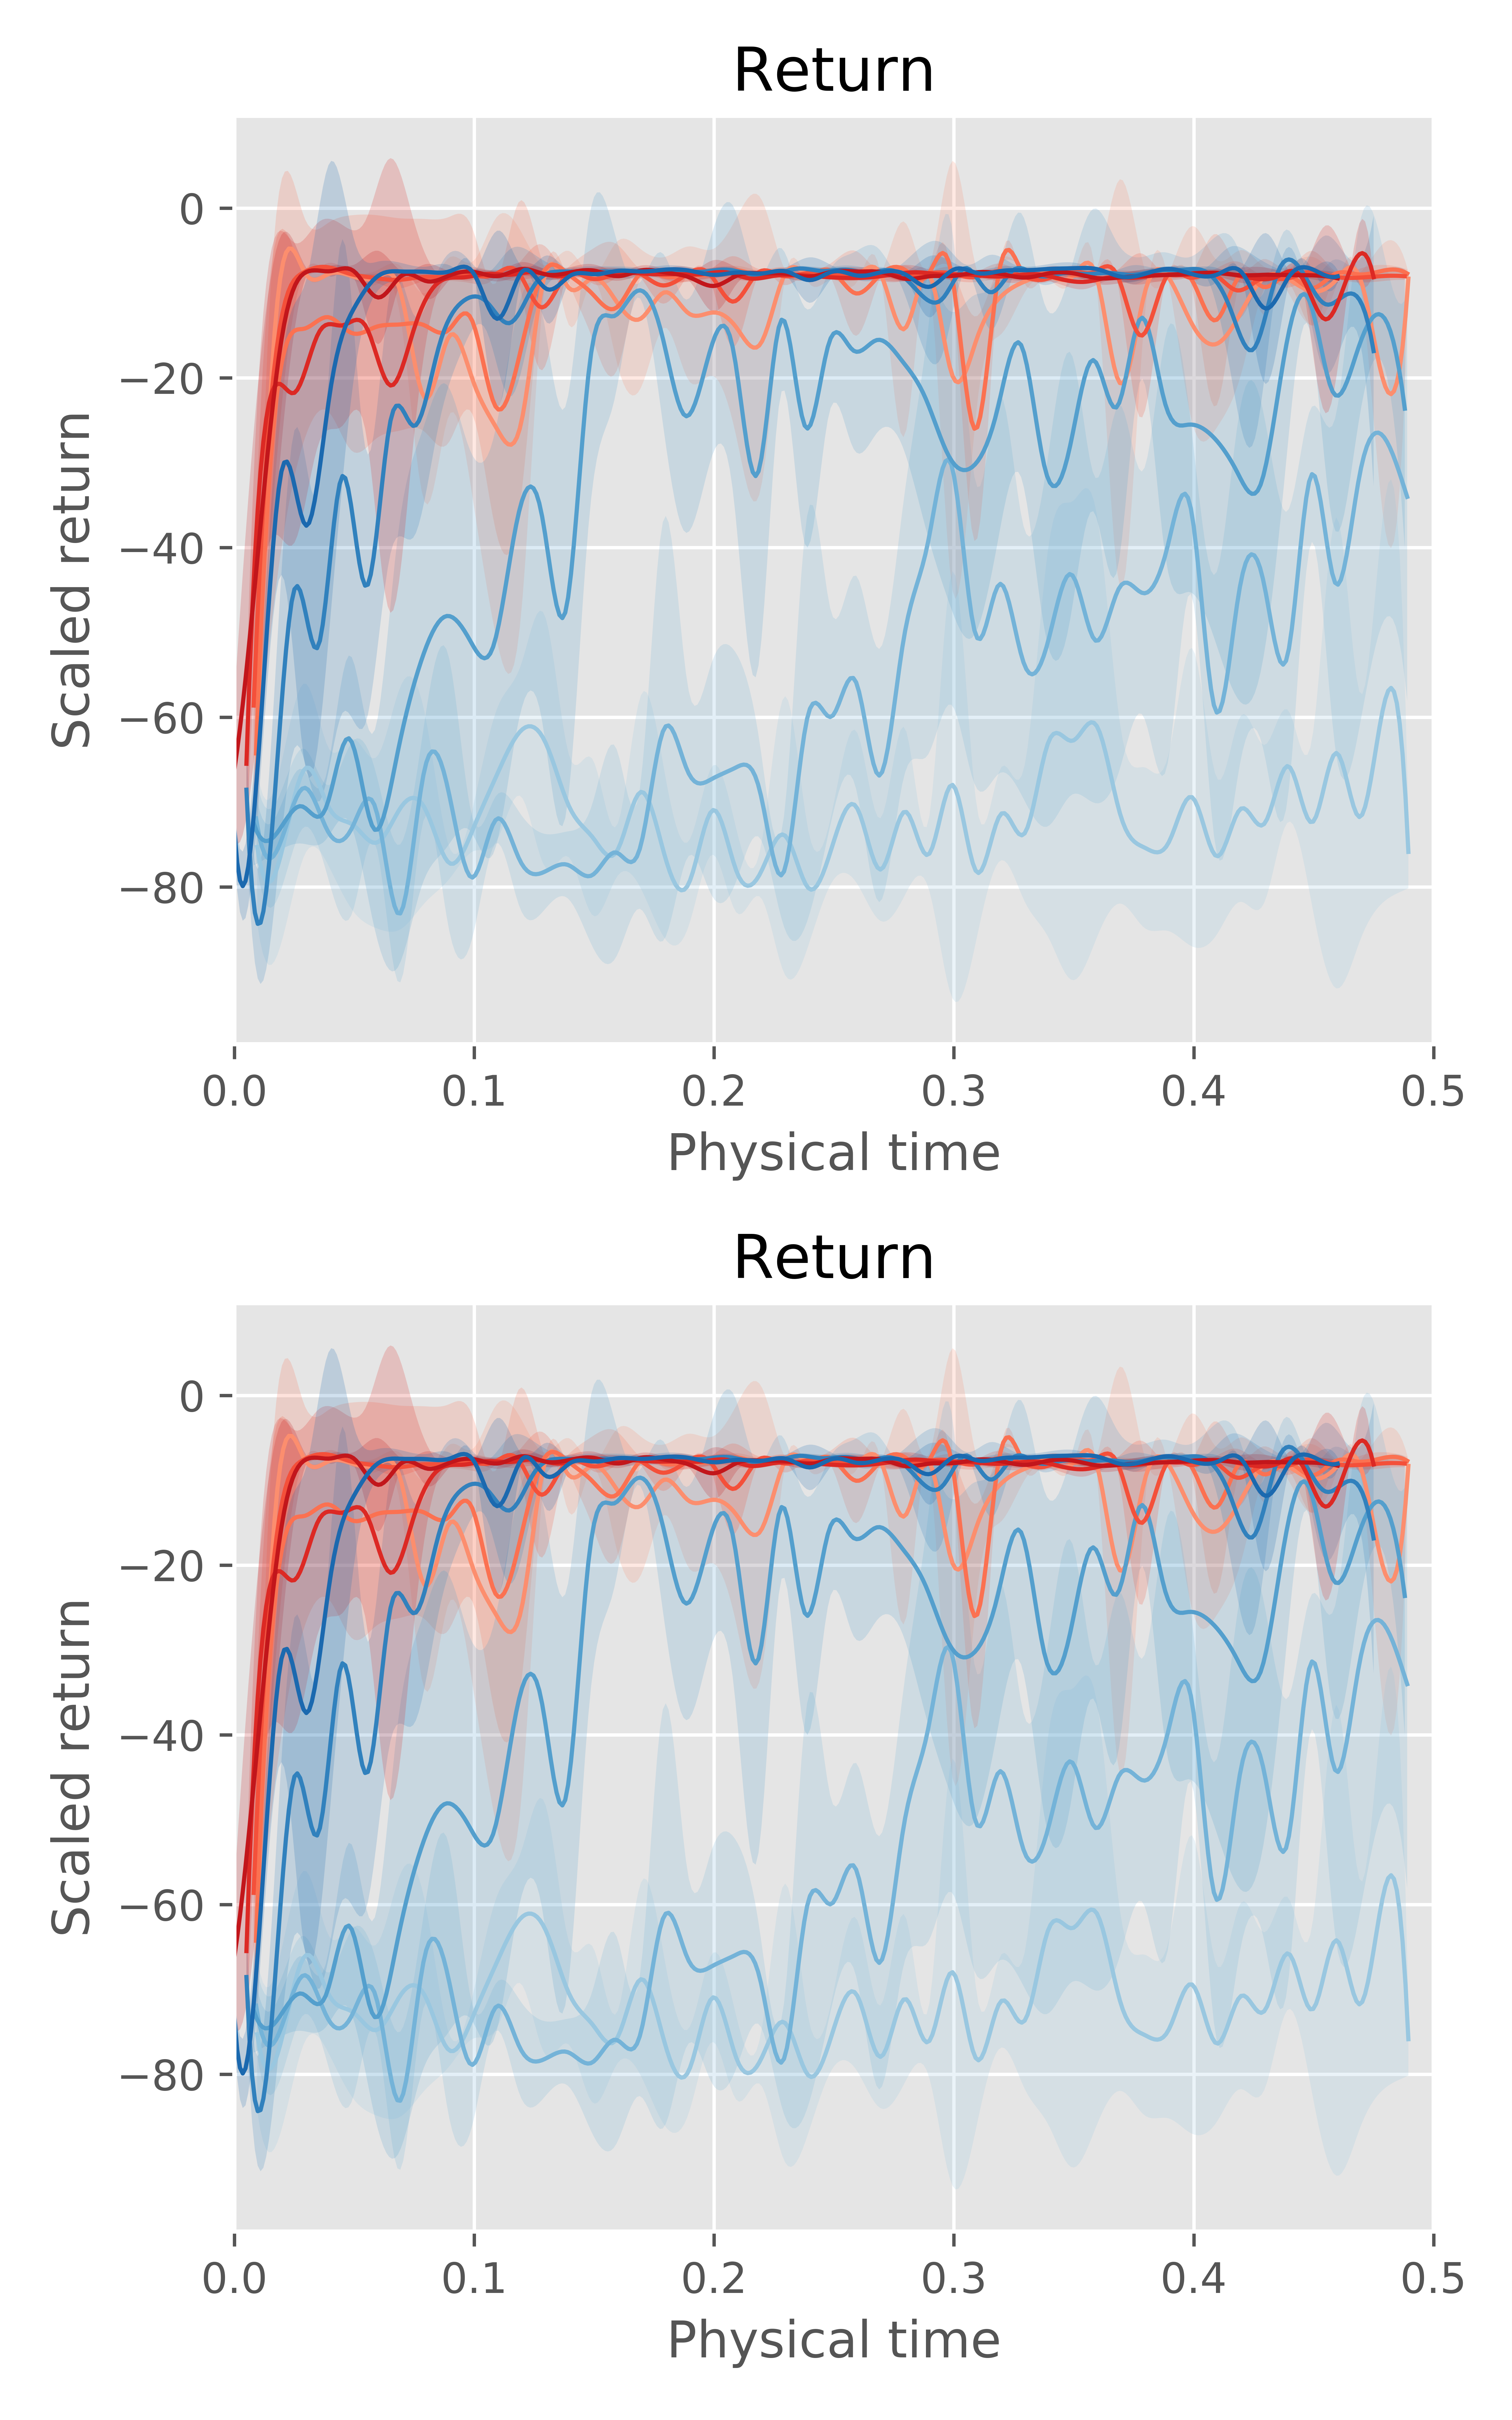
\includegraphics[width=\columnwidth]{figs_data/pendulum_lc.png}
%   \caption{Pendulum}
%   \label{fig:pendulum-lc}
% \end{figure}
